\section{Result}

\subsection{Simulation of indexes}
\begin{frame}
\myframetitle{}
Simulation of S\&P500 and Nikkei225 using GBM process:
\begin{itemize}
	\item S\&P500 $\sigma = 23 \%$ \\
	\begin{center}
	\vspace{0.3cm}
	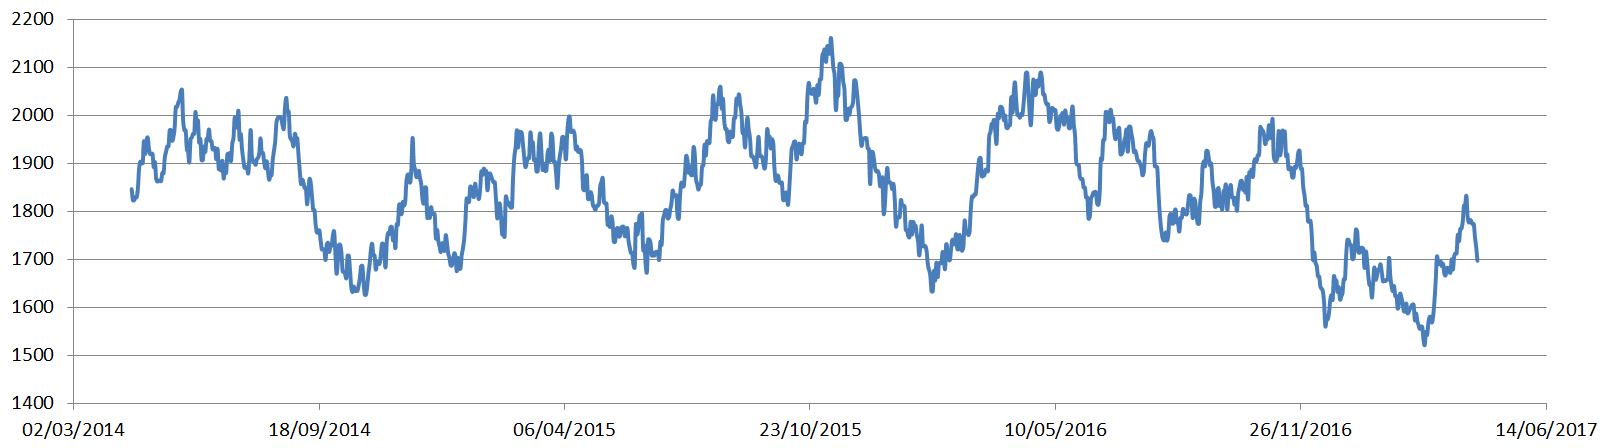
\includegraphics[width=0.7\linewidth]{../Report/SandP500_simulated}
	\end{center}
	\item Nikkei225 $\sigma = 43 \%$\\
	\begin{center}
	\vspace{0.3cm}
	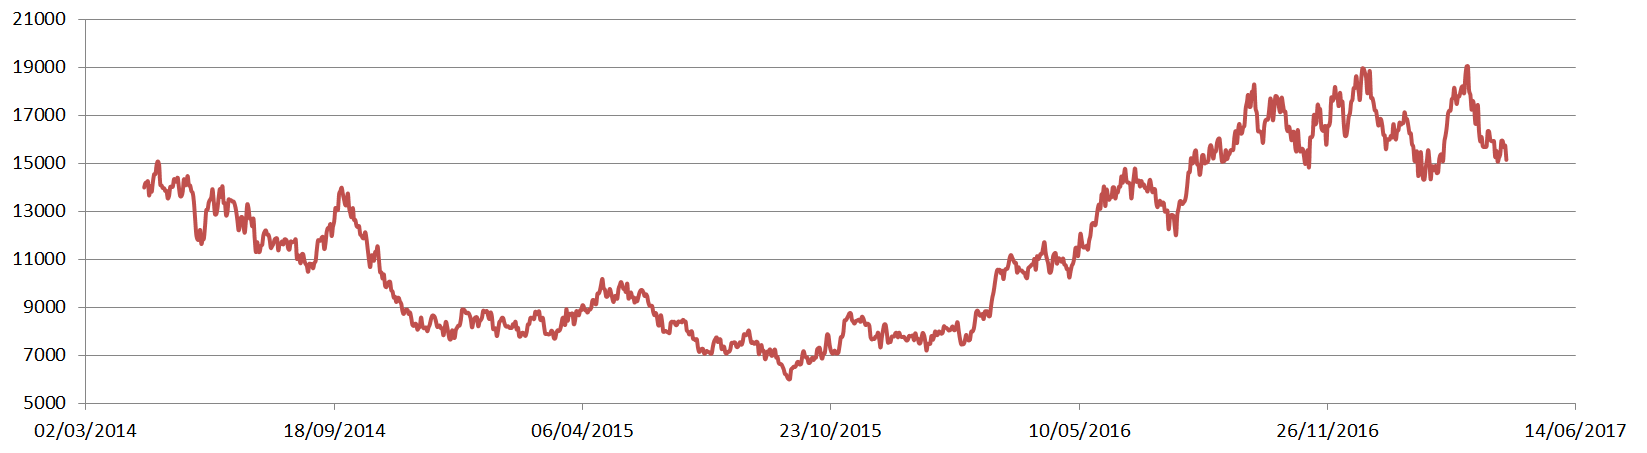
\includegraphics[width=0.7\linewidth]{../Report/Nikkei225_simulated}
	\end{center}
	
\end{itemize}
\end{frame}

\subsection{Expected return}
\begin{frame}[c]
\myframetitle{}
Estimation of the financial product return
\begin{itemize}
	\item Mean return : -26.1 \%
	\item Variance :  8,9 \%
\end{itemize}

\vspace{1cm}

\begin{itemize}
\item For an investment of 100 in this financial product, the expected amount returned is 73.9.
\end{itemize}

\end{frame}

\subsection{Probability of loss}
\begin{frame}
\myframetitle{}
Cumulative density function of the return: \\
\vspace{0.5cm}
\centering
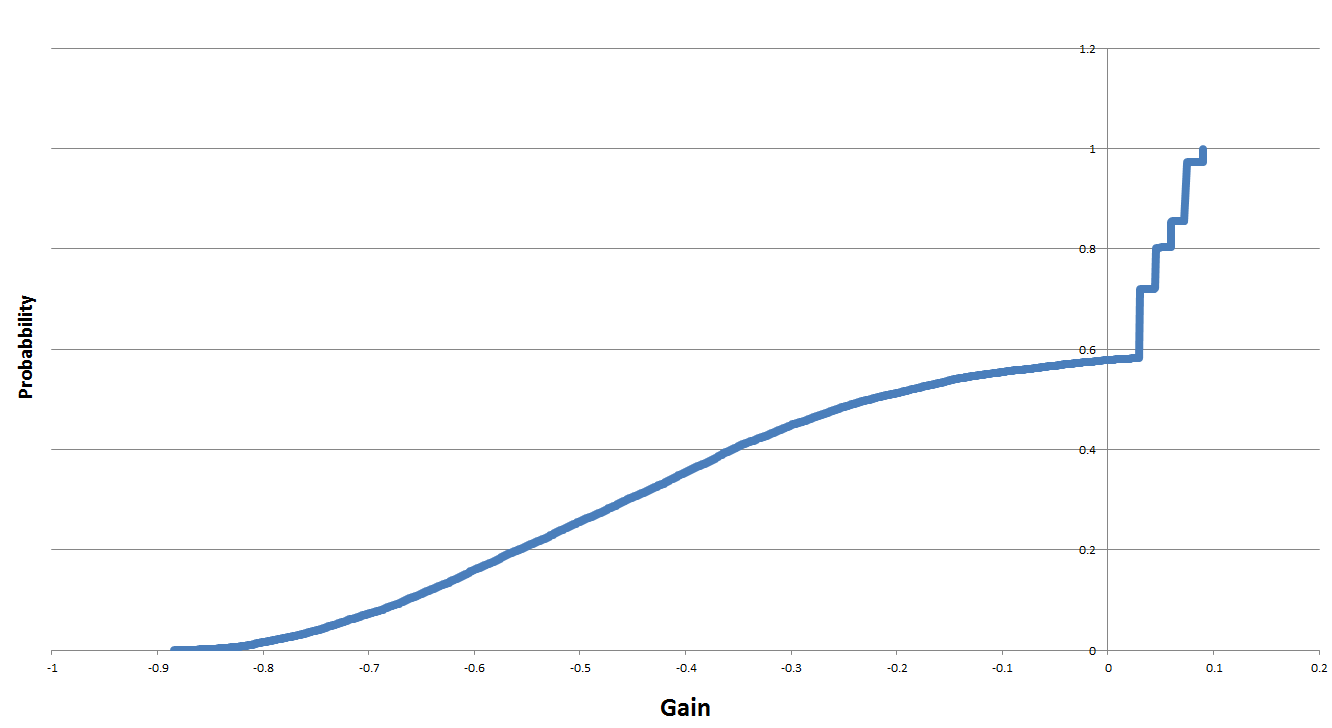
\includegraphics[width=0.9\linewidth]{../Report/Gain}
\begin{itemize}
\item The investor has less than half a chance to get a positive return with this product
\end{itemize}
\end{frame}



\subsection{Numerical efficiency}
\begin{frame}
\myframetitle{}
Mean and variance depending on the number of samples
\begin{figure}
	\centering
	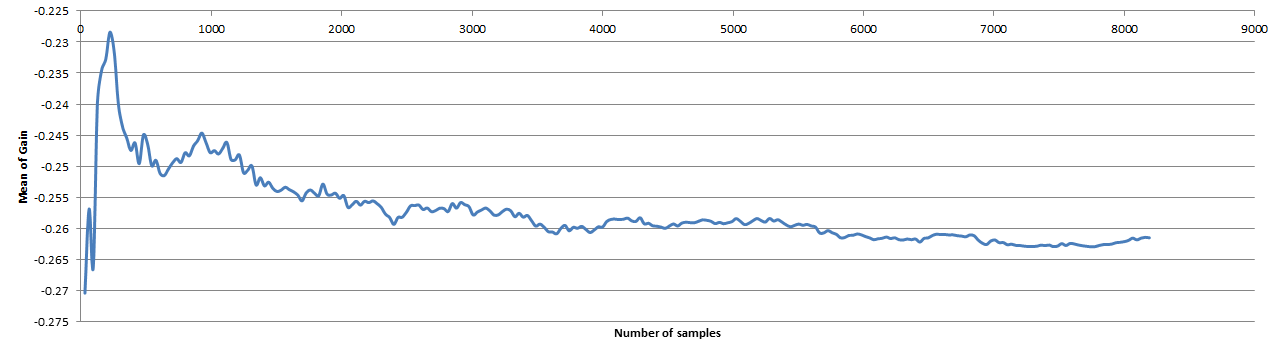
\includegraphics[width=0.9\textwidth]{../Report/Mean_of_the_gain} \\
	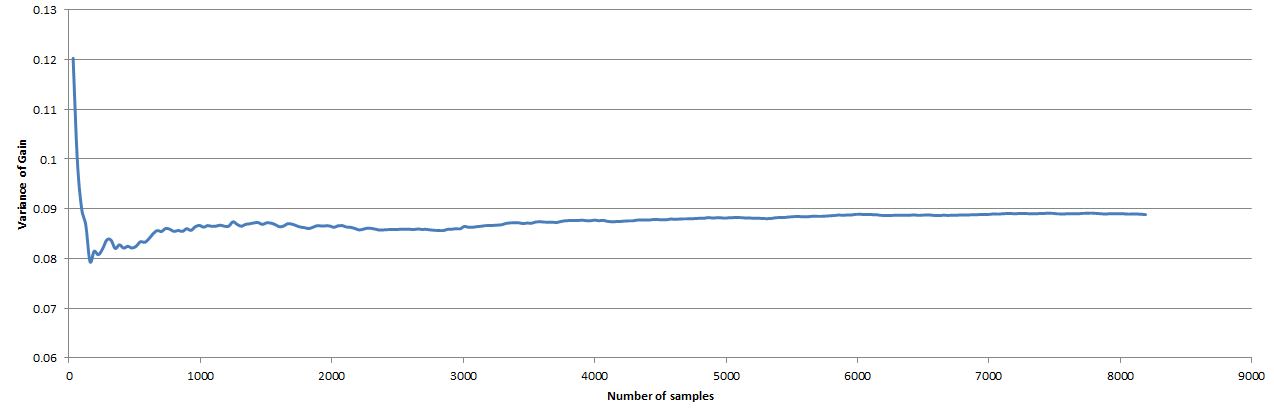
\includegraphics[width=0.9\textwidth]{../Report/Variance_of_the_gain}
\end{figure}
\end{frame}

\subsection{Sensitivity analysis}
\begin{frame}
\myframetitle{}
Return for different Knock-in value:
\begin{itemize}
	\item Mean and Variance \\
	\begin{center}
	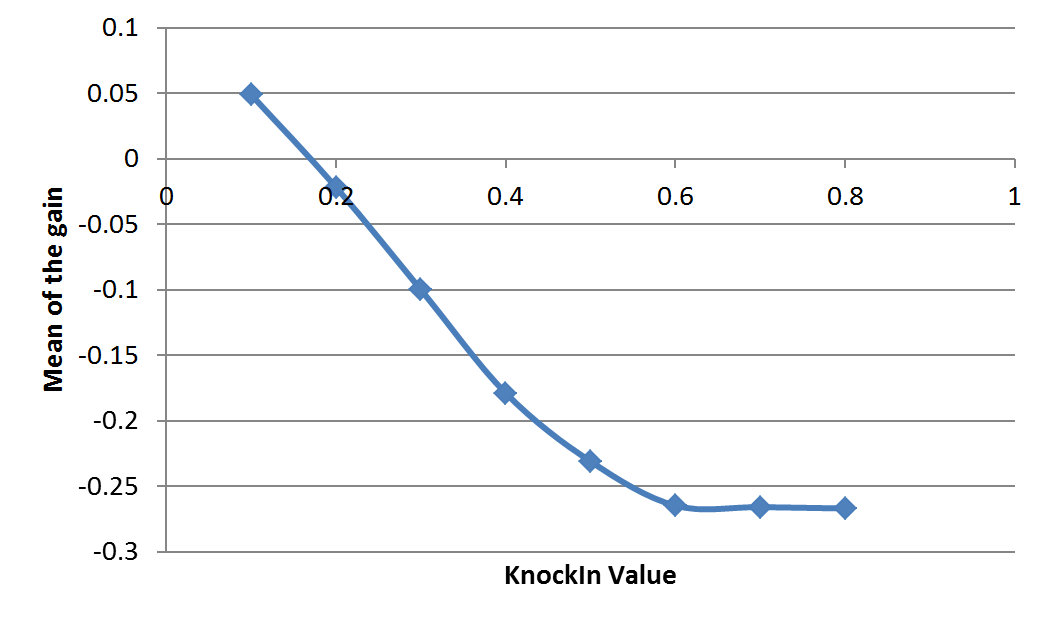
\includegraphics[width=0.3\textwidth]{../Report/Mean_depending_on_knockin}
	\hspace{2cm}
	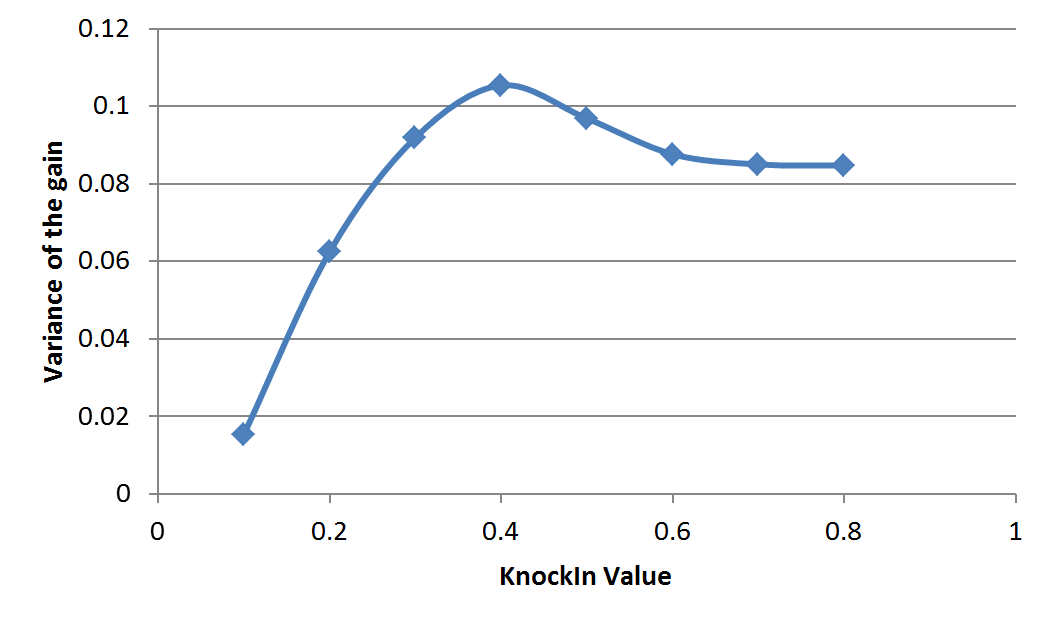
\includegraphics[width=0.3\textwidth]{../Report/Variance_depending_on_knockin}
	\end{center}
	\item CDF comparison \\
	\centering
	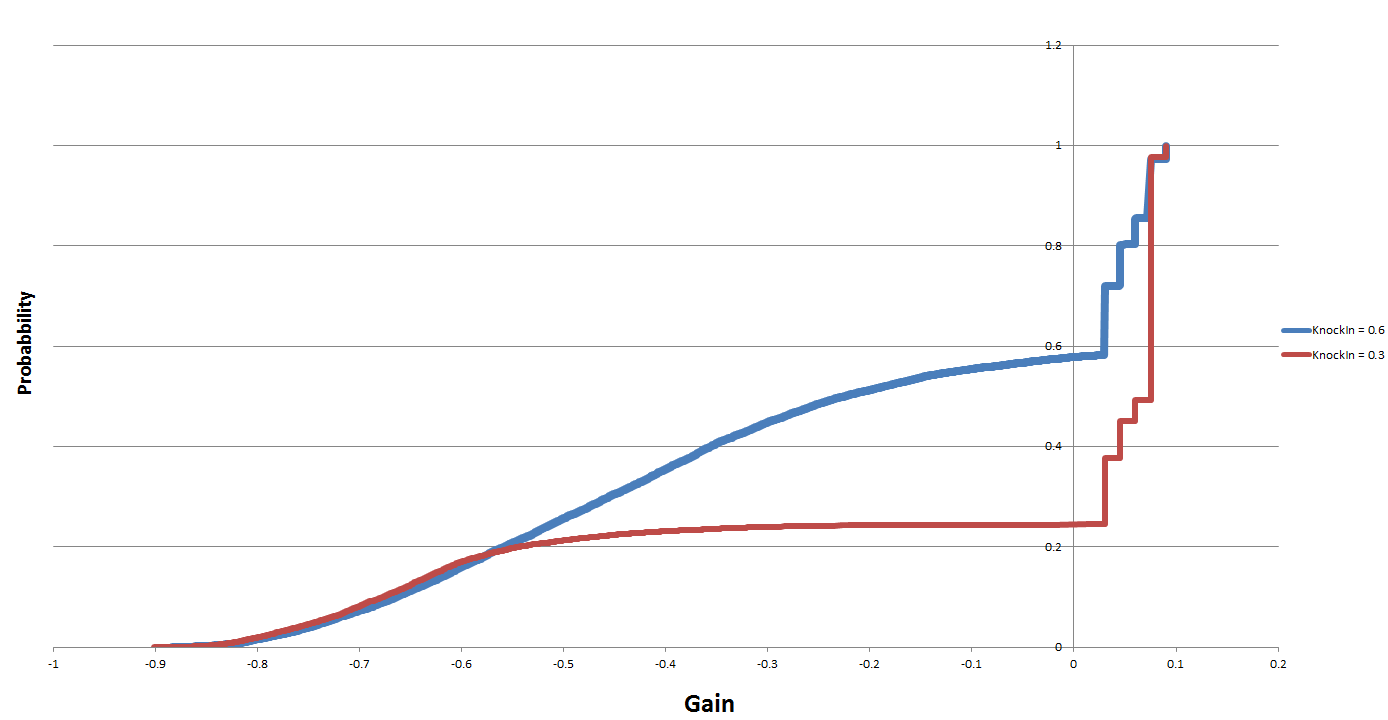
\includegraphics[width=0.5\textwidth]{../Report/KnockInCDFComparaison}
\end{itemize}
\end{frame}

\begin{frame}[c]
\myframetitle{}
\begin{itemize}
	\item A possible way to make this product fair would be to set:
	\begin{itemize}
			\item the knock-in value around 20 \% (non realistic)
			\item the interest rate to 14 \%
	\end{itemize}
	\item Removing the knock-out makes the product less valuable for the investor (-32 \%)
	\item For a knock-in value of 30 \% we can make the following comments: \\
	\begin{itemize}
		\item Daiwa still makes a profit which is around 10 \% of the investment
		\item The probability of gain for the investor is around 80 \% which could be an interesting commercial argument
	\end{itemize}
\end{itemize}
\end{frame}

%\subsection{Comparison with Product A}
%\begin{frame}
%\myframetitle{}
%\begin{itemize}
%	\item 2 indexes : EuroSTOXX50 \& Nikkei225, T = 5 years, Knock-out 49\% 
%	$$
%	r = 
%	\left \{
%	\begin{array}{ll}
%    1\%   & \mbox{if one of the index is under 80\% of its initial value} \\
%		5.7\% & \mbox{else, or it is the first interest payment}
%  \end{array}
%	\right.
%	$$
%\end{itemize}
%\end{frame}